\documentclass[12pt]{article}
% \textwidth 15.5cm \oddsidemargin 0cm \topmargin -2cm \textheight
% 24cm \footskip 1cm
\usepackage[british]{babel}
\usepackage{epsfig}
\usepackage{amsmath,graphicx,psfrag,pstricks,float,amssymb,fancyhdr,pdfpages, hyperref, enumitem, listings, subcaption, minted, diagbox, appendix, lastpage, biblatex, bm}
% \usepackage[sorting=none]{biblatex}
\usepackage[margin=25mm]{geometry}

\DeclareMathOperator*{\argmax}{argmax}
\DeclareMathOperator*{\argmin}{argmin}

% \pagestyle{fancy}
% \pagenumbering{arabic}
% \fancyhead[L]{}
% \cfoot{\thepage}
\fancypagestyle{technical_abstract}{
  \fancyhf{}
  \fancyfoot[C]{Page \thepage}
}

\fancypagestyle{default}{
  \fancyhf{}
  \fancyfoot[C]{Page \thepage\ of \pageref{LastPage}}
}

\pagestyle{fancy}

% \setlength{\headheight}{15pt}
\renewcommand{\headrulewidth}{0pt}
\linespread{1.3}  % "One-and-a-half" spacing

\def\n{\noindent}
\def\u{\underline}
\def\hs{\hspace}
\newcommand{\thrfor}{.^{\displaystyle .} .}
%\newcommand{\bvec}[1]{{\bf #1}}

\addbibresource{bibliography.bib}

\begin{document}

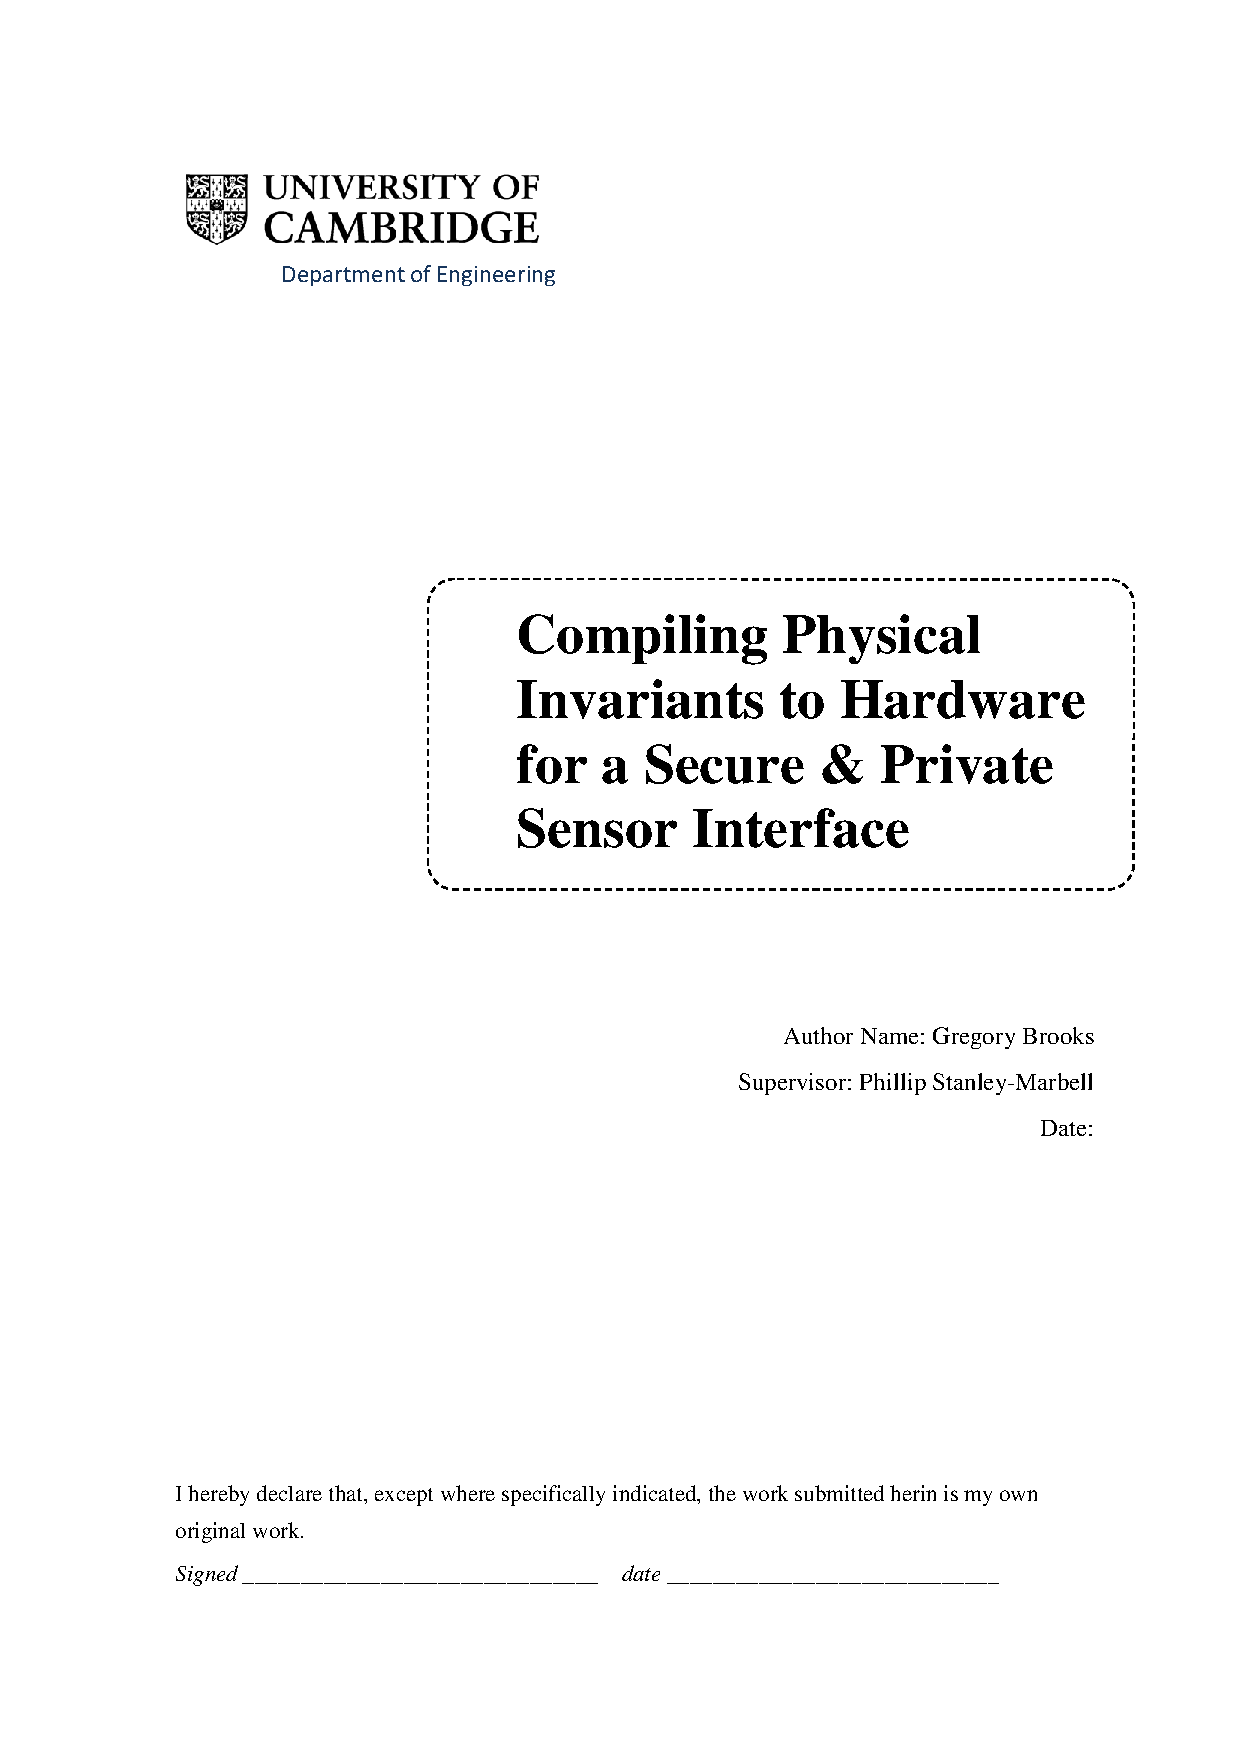
\includepdf[pages={1}]{coversheet.pdf}
\clearpage \mbox{}
\pagenumbering{gobble}
\clearpage
\pagenumbering{arabic}

\noindent

%
% TITLE & CONTENTS PAGE
%

\title
{
  IIB Project Report:\\
  Compiling Physical Invariants to Hardware for a Secure \& Private Sensor Interface\\
}
\author{Gregory Brooks, gb510, Christ's College}
\date{}
\maketitle

\tableofcontents

\pagenumbering{gobble}
\clearpage
\pagenumbering{arabic}

%
% TECHNICAL ABSTRACT
%
\pagestyle{technical_abstract}
\section{Technical Abstract}

\begin{center}
{
  \bf Compiling Physical Invariants to Hardware for a Secure \& Private Sensor Interface\\
}
Gregory Brooks, gb510, Christ's College
\end{center}
\rule{15.7cm}{0.5mm}
\vspace{1cm}

  %
  % SYSTEM DIAGRAM
  %

  \subsection{System Diagram}
    \textit{$\langle$ TODO: insert block diagram of system and describe which parts have been the focus of this project$\rangle$}

  \textit{$\langle$ TODO: write this last$\rangle$}

\newpage


\pagestyle{default}
%
% INTRODUCTION
%

\section{Introduction}

\newpage



%
% THEORRTICAL DEVELOPMENT
%

\section{Theoretical Development}

  \subsection{Brainstorming Example Applications}
    \subsubsection{\textit{Intelligent} Noising}
      \textit{$\langle$ TODO: allowing the compiler to choose how to add noise, rather than explicity stating where to add noise$\rangle$}

    \subsubsection{Digital Camera/Viola-Jones Facial Detection}

    \subsubsection{Microphone}


  \subsection{System Specification}
    \textit{$\langle$ TODO: move to technical abstract?$\rangle$}

  \subsection{Multi-Sensor Differential Privacy Loss}

  \subsection{Privacy Budget Management Algorithm}

\newpage



%
% APPARATUS, EQUIPMENT AND TECHNIQUES
%

\section{Apparatus, Equipment and Techniques}

  \subsection{iCE40 FPGA}

  \subsection{Software Prototyping}

  \subsection{FPGA Synthesis}

  \subsection{Repository Structure and Build System}

  \subsection{Verilog Development Techniques}
    \textit{$\langle$ TODO: describe good practices picked up over the course of this project$\rangle$}

\newpage



%
% DELIVERABLES
%

\section{Deliverables}
  \subsection{Hardware Entropy Source}
    One of the key components of a security/privacy application is a true random number generator (TRNG). Unlike a pseudorandom number generator (PRNG), which produces a predictable deterministic outcome, a true random number generator's output cannot be anticipated by an attacker, preserving system security and users' privacy. The output rate of TRNGs is often limited so can be used to seed a cryptographically secure PRNG (CSPRNG) algorithm to increase output data rate without significantly compromising security. This extra step was not required for this project, since the rate at which random numbers are consumed is relatively low.

    I investigated using the iCE40 FPGA's hardware to generate \textit{$\langle$ TODO: finish$\rangle$}

  \subsection{Uniform Random Number Generator}
  \textit{$\langle$ TODO: insert block diagram$\rangle$}

  \subsection{Inversion Method Random Number Generator}
    \textit{$\langle$ TODO: insert block diagram$\rangle$}



%
% RESULTS
%

\section{Results}

  \subsection{Scaling of Logic Implementations}
    \textit{$\langle$ TODO: investigate how URNG and RNG logic implementations scale with various parameters (and how this compares to a naive implementation)$\rangle$}

  \textit{$\langle$ TODO: investigate scaling of adder hardware (inferred from Verilog vs iCE40 hardware accumulators)$\rangle$}

\newpage



%
% CONCLUSIONS
%

\section{Conclusions}

\newpage



\noindent

% Hack to remove REFERENCES REFERENCES header
\markboth{}{}
\printbibliography
\markboth{}{}

\newpage

\begin{appendix}

  %
  % RISK ASSESSMENT RETROSPECTIVE
  %

  \section{Risk Assesment Retrospective}
    The risk assessment submitted at the start of the project does not mention any specific hazards besides office (computer) work, since the project is predominately software/firmware based (all project hardware operated at low voltages i.e. 12V or less). No other hazards were encountered during the course of the project, since the random noise generator PCBs were manufactured by the Dyson Centre's Electronics Development Group. In retrospect, although not part of the initial project specification, the risk assessment could have anticipated the possibility of manufacturing PCBs for the project. The hazards associated with this activity include high temperatures (from a soldering iron/oven/hot air gun) as well as chemical hazards associated with solder, fume extraction etc.



  %
  % UPPER BOUND ON DIFF PRIV
  %

  \section{Derivation of an Upper Bound on \textit{Indirect} Differential Privacy Loss}
    Let $\hat{X}$ be a random variable denoting a sensor measurement, including any measurement error.
    \\
    \\
    Let $X$ be a random variable representing a \textit{noised} sensor measurement i.e. the masked value that the differential privacy system provides to the outside world after applying Laplace distributed noise to a measurement:

    \begin{equation}
      X = \hat{X} + N_{Laplace}
    \end{equation}
    \\
    A measurement event comprises the variable $\hat{X}$ taking on value $\hat{x}_i$. Similarly, a noising event can be defined by $X$ taking value $x_i = \hat{x}_i + n_i$.
    \\
    \\
    Let $Y$ denote a variable derived from one or more $X$ variables, such as measurements from different sensors in an embedded system:
    \begin{align*}
      Y & = f(X_1, X_2, ..., X_n) = f(\bf{X})\\
      y_i & = f(x_{i1}, x_{i2}, ..., x_{in}) = f(\bf{x_i})
    \end{align*}
    \\
    This same mapping function $f(\bf{x})$ can take unnoised measurements as arguments:
    \begin{align*}
      \hat{Y} & = f(\hat{X}_1, \hat{X}_2, ..., \hat{X}_n) = f(\bf{\hat{X}})\\
      \hat{y}_i & = f(\hat{x}_{i1}, \hat{x}_{i2}, ..., \hat{x}_{in}) = f(\bf{\hat{x}_i})
    \end{align*}
    \\
    If measurements $x_{i1}$ to $x_{in}$ are taken, a value for $y_i$ can be computed from them --- variable $Y$ has experienced some privacy loss, $l_Y$ that can be calculated as a log-likelihood ratio~\cite{Choi2018GuaranteeingLD} (Equation \ref{eqn:privacy_loss}). This privacy loss function requires two parameters,  $\hat{y}_a$ and $\hat{y}_b$, which are the possible \textit{true} i.e. unnoised values for $\hat{Y}$ that maximise the privacy loss (Equation \ref{eqn:argmax}).
    \begin{equation}
      y_{obs} = f(\bf{x}_{obs}) = \text{value for $y$ calculated from noised measurements $\bf{x}_i$} \nonumber\\
    \end{equation}
    \begin{align}
      % \bf{\hat{x}_a}, \bf{\hat{x}_b} & = \argmax_{\bf{\hat{x}_a}, \bf{\hat{x}_b}} l_Y(\bf{\hat{x}_a}, \bf{\hat{x}_b}) \label{eqn:argmax}\\
      % l_Y(\bf{\hat{x}_a}, \bf{\hat{x}_b}) & = log \left( \frac{Pr\{ Y = y_{obs} | \bf{\hat{X}} = \bf{\hat{x}_a} \}}{Pr\{ Y = y_{obs} | \bf{\hat{X}} = \bf{\hat{x}_b} \}} \right) \label{eqn:privacy_loss}
      \hat{y}_a, \hat{y}_b & = \argmax_{\hat{y}_a, \hat{y}_b} l_Y(\hat{y}_a, \hat{y}_b) \label{eqn:argmax}\\
      l_Y(\hat{y}_a, \hat{y}_b) & = log \left( \frac{Pr\{ Y = y_{obs} | \hat{Y} = \hat{y}_a \}}{Pr\{ Y = y_{obs} | \hat{Y} = \hat{y}_b \}} \right) \label{eqn:privacy_loss}
    \end{align}
    \\
    Equation \ref{eqn:privacy_loss} can be rewritten as follows, where $\bf{\hat{x}_a}$ and $\bf{\hat{x}_b}$ are chosen to maximise $l_Y$ as before, but subject to constraints $\bf{\hat{x}_a}$ $ = f^{-1}(\hat{y}_a)$ and $\bf{\hat{x}_b}$ $ = f^{-1}(\hat{y}_b)$:
    \begin{align}
      l_Y(\bf{\hat{x}_a}, \bf{\hat{x}_b}) & = log \left( \frac{Pr\{ \bf{X} = \bf{x}_{obs} | \bf{\hat{X}} = \bf{\hat{x}_a} \}}{Pr\{ \bf{X} = \bf{x}_{obs} | \bf{\hat{X}} = \bf{\hat{x}_b} \}} \right)
    \end{align}
    \\
    This constrained optimisation problem could be solved to calculate an exact value for privacy loss. Alternatively, an upper bound on privacy loss can be determined using a far simpler calculation:
    \begin{align}
      l_Y(\bf{\hat{x}_a}, \bf{\hat{x}_b}) & = log \left( \prod_{u=1}^n \frac{Pr\{ X_u = x_{u,obs} | \hat{X}_u = \hat{x}_{u,a} \}} {Pr\{ X_u = x_{u,obs} | \hat{X}_u = \hat{x}_{u,b} \}} \right) \nonumber \\
      & \leq log \left( \prod_{u=1}^n \frac{Pr\{ X_u = x_{u,obs} | \hat{X}_u = \hat{x}_{u,c} \}}{Pr\{ X_u = x_{u,obs} | \hat{X}_u = \hat{x}_{u,d} \}} \right) \label{eqn:upper_bound} \\
      \text{where:} & \nonumber \\
      & \hat{x}_{u,c} = \argmax_{\hat{x}_{u,c}}Pr\{ X_u = x_{u,obs} | \hat{X}_u = \hat{x}_{u,c} \} \nonumber \\
      & \hat{x}_{u,d} = \argmin_{\hat{x}_{u,d}}Pr\{ X_u = x_{u,obs} | \hat{X}_u = \hat{x}_{u,d} \} \nonumber
    \end{align}
    i.e. the constraint $f^{-1}(\hat{y})$ has been removed. Equation \ref{eqn:upper_bound} can be interpreted as the sum of the privacy losses incurred by the $X$ variables i.e. $\sum_{u=1}^n l_{X_u}$.
    \\
    \\
    Since the Newton language recently gained a mutual information operator, I attempted to factor mutual information into this calculation. Unfortunately, it appears that mutual information alone does not provide enough information to calculate indirect privacy loss --- the exact nature of the correlation between two (or more) random variables is required i.e. the conditional distribution for the unknown variable given known ones:

    \textit{$\langle$ TODO: include working here$\rangle$}


  %
  % URNG BLOCK DIAGRAM
  %

  \section{Uniform Random Number Generator: Block Diagram}
    \textit{$\langle$ TODO: insert block diagram$\rangle$}


  %
  % INVERSION METHOD BLOCK DIAGRAM
  %

  \section{Inversion Method Random Number Generator: Block Diagram}
    \textit{$\langle$ TODO: insert block diagram$\rangle$}


  %
  % NOISE GENERATOR SCHEMATIC AND PCB LAYOUT
  %
  \newpage
  \section{Hardware Entropy Source Schematic and PCB}
    \begin{figure}[H]
      \centering
      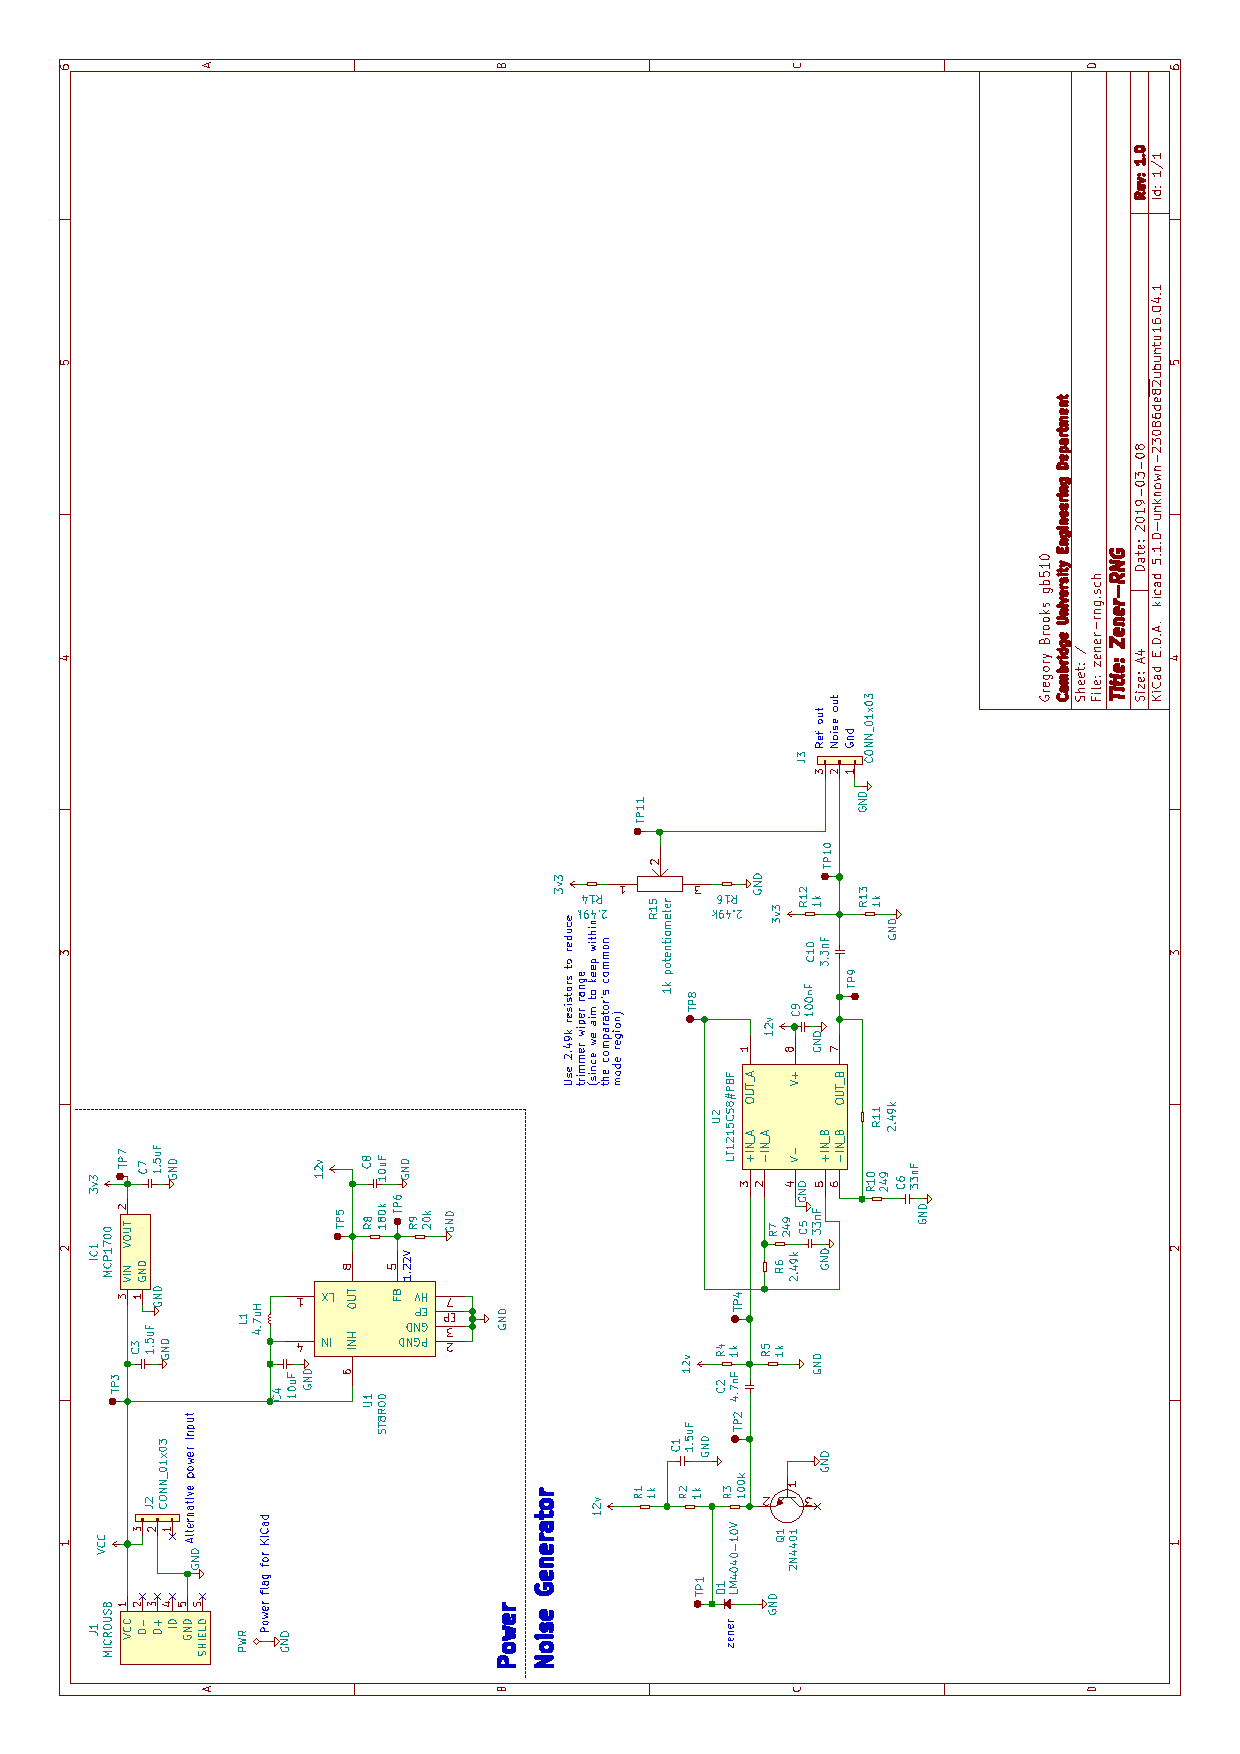
\includegraphics[width=\textwidth]{schematic.pdf}
      \label{fig:schematic}
    \end{figure}

  %
  % EUROSYS POSTER
  %

  \section{EuroSys 2019 Poster: Safeguarding Sensor Device Drivers Using Physical Constraints}
    \subsection{Description}
      This poster~\cite{eurosys_poster} was submitted to EuroSys 2019, to communicate the idea of using information about a physical system to condition electronic sensor measurements. The example discussed in the poster is the detection and safeguarding against transduction attacks~\cite{Fu_2018}, where an attacker manipulates a sensor's output to gain control over a system. For example, a presentation~\cite{autonomous_vehicles} illustrates how the proximity sensors on a Tesla vehicle can be fooled into providing erroneous (or even no) data using ultrasonic interference produced by a device built using off-the-shelf electronics. An attacker would not need to have access to the Tesla software (or even physical access to the hardware) in order to control the system's behaviour.

      The poster illustrates how the Newton language can be used to describe a physical system, in this case an accelerometer mounted to a PCB without vibration isolation. In this scenario, vibrations of the PCB (e.g. due to a nearby loudspeaker or even, in the case of a smartphone, due to loudspeakers mounted to the PCB) are measured by the accelerometer, obscuring a \textit{true} acceleration measurement. This effect is particularly pronounced if the board is driven at its resonant frequency, since the resulting oscillation will have a greater amplitude~\cite{adi}. This phenomenon could, in theory, be used as part of a transduction attack e.g. where a smartphone's loudspeaker is used to interfere with an application's estimate of the device's physical orientation.

      To test whether this phenomenon can be distinguished from regular measurement noise, an experiment~\cite{poster_experiment} was performed using an MMA8451Q accelerometer mounted on an FRDM-KL03Z board. With the sensor resting on a desk, five minutes worth of accelerometer samples were recorded at 10Hz in order to obtain a probability distribution for the accelerometer's measurement noise (along the z axis, aligned with the vertical); this data was empirically observed to fit a Laplace distribution. This measurement was then repeated with the board resting on top of a smartphone playing a 440Hz audio tone --- in theory, this data (random samples from a sinusoid) would fit a bimodal beta distribution (derivation in section \ref{Poster_Derivation}) allowing a log likelihood ratio to be computed:

      \begin{equation}
        LLR = -2 \sum_{i = 1}^{N} \frac{\frac{1}{\pi}\left| \frac{1}{\sqrt{A^2\omega^4 - \ddot{x}_i^2}} \right|}{\frac{1}{2b} exp\left(-\frac{|\ddot{x}_i-\mu|}{b}\right)}
      \end{equation}

      For the data collected in the experiment, the log-likelihood ratio was found to be around -24600.08; the negative value indicates that the measurements taken whilst the tone was playing were indeed more accurately described by the bimodal beta distribution, compared to the Laplace distribution of sensor noise. Computing this log-likelihood ratio could therefore be used as evidence to suggest whether an audio tone based transduction attack is in progress.

    \subsection{Derivation of Bimodal Beta Distribution} \label{Poster_Derivation}
    Let T be a uniformly distributed random variable representing the time at which acceleration is sampled:
    \begin{align}
      T & \sim U\left(-\frac{\pi}{\omega}, \frac{\pi}{\omega}\right) \nonumber \\
      f_T(t) & =
        \begin{cases}
          \frac{\omega}{2\pi} & -\frac{\pi}{\omega} \leq t \leq \frac{\pi}{\omega}\\
          0 & \text{otherwise}
        \end{cases}\\
      F_T(t) & =
        \begin{cases}
          0 & t < -\frac{\pi}{\omega}\\
          \frac{\omega (t + \pi / \omega)}{2\pi} & -\frac{\pi}{\omega} \leq t \leq \frac{\pi}{\omega}\\
          1 & t > \frac{\pi}{\omega}
        \end{cases}
    \end{align}
    Then let X = g(T) represent the acceleration value at time T. By considering the dynamics of the system, we know that:

    \begin{equation}
      g(t) = A \omega^2 sin(\omega t)
    \end{equation}
    where A is a frequency-dependent constant (equal to the product of quality factor and board displacement at resonance). We can also define a monotonically increasing function $h(x)$ as the inverse of $g(t)$:

    \begin{equation}
      h(x) = g^{-1}(x) = \frac{1}{\omega} arcsin \left(\frac{x}{A\omega^2}\right)
    \end{equation}
    \\
    The cumulative distribution function for X can therefore be written in terms of the cumulative distribution function for T, accounting for the fact that g(t) is not monotonic:
    \begin{equation}
      F_X(x) = F_T(h(x)) + \Big(1 - F_T(\pi/\omega - h(x))\Big)
    \end{equation}
    \\
    Taking the derivative results in the probability density function for X:
    \begin{align}
      f_X(x) & = \Big(f_T(h(x) - f_T(-h(x)))\Big) \frac{d(h(x))}{dx}\\
      & =
      \begin{cases}
        \frac{1}{\pi \sqrt{A^2 \omega^4 - x^2}} & |x| \leq A \omega^2\\
        0 & \text{otherwise}
      \end{cases}
    \end{align}


    \subsection{Poster}
      \textit{$\langle$ TODO: insert the poster into this report?$\rangle$}

\end{appendix}

\end{document}
